%% Refer elsdoc for options available for "Document Class"
\documentclass[3p]{elsarticle}

%% \usepackage{lineno}
\usepackage{lineno,hyperref}
% if you have landscape tables
\usepackage[figuresright]{rotating}

%% Custom Packages
%%\usepackage{fixltx2e} %% For SubScript
\usepackage{float} %% For image placement

%% Put line numbers for every line.
\modulolinenumbers[1] 

%% Enter Journal Name here
\journal{Materials and Design}
%%%%%%%%%%%%%%%%%%%%%%%%%%%%%%%%%%%%%%%%%%%%%%%%%%%%%%%%%%%%%%%%%%%%%%%%%%

%% The amssymb package provides various useful mathematical symbols
\usepackage{amssymb} 
%% The amsmath package provides various useful mathematical formulae
\usepackage{amsmath}
%% The amsthm package provides extended theorem environments
%% \usepackage{amsthm}

%%%%%%%%%%%%%%%%%%%%%%%
%% Reference Styling %%
%%%%%%%%%%%%%%%%%%%%%%%

%% natbib.sty is loaded by default. However, natbib options can be
%% provided with \biboptions{...} command. Following options are
%% valid:

%%   round  -  round parentheses are used (default)
%%   square -  square brackets are used   [option]
%%   curly  -  curly braces are used      {option}
%%   angle  -  angle brackets are used    <option>
%%   semicolon  -  multiple citations separated by semi-colon
%%   colon  - same as semicolon, an earlier confusion
%%   comma  -  separated by comma
%%   numbers-  selects numerical citations
%%   super  -  numerical citations as superscripts
%%   sort   -  sorts multiple citations according to order in ref. list
%%   sort&compress   -  like sort, but also compresses numerical citations
%%   compress - compresses without sorting
%%
%% Example : \biboptions{comma,round}

\biboptions{square,comma,sort&compress}
%%%%%%%%%%%%%%%%%%%%%%%%%%%%%%%%%%%%%%%%%%%%%%%%%%%%%%%%%%%%%%%%%%%%%%%%%%
                   %% Declarations for front matter
\begin{document}
                   %% Declarations of Commands
\newcommand{\degree}{\ensuremath{^{\circ}}}  %% Command for degree


\begin{frontmatter}

\title{Friction welding of Ti-6Al-4V tube to AA6061 tube-plate using an external tool}

%%%%%%%%%%%%%%%%%%%%%%%%%%%%%%%%%%%%%%%%%%%%%%%%%%%%%%%%%%%%%%%%%%%%%%%%%%
                      %% Author Declaration
\author[META]{Sharan. C}
\ead{Sharanc25@gmail.com}
\author[META]{Maxwell Rejil. C}
\ead{maxwellrejilc@gmail.com}
\author[META]{Sooraj. R}
\ead{soorajramana89@gmail.com}
\author[META]{Muthukumaran. S\corref{cor1}}
\ead{smuthu@nitt.edu}
%\ead[url]{http://www.nitt.edu/home/academics/departments/meta/faculty/asstprof/smuthu}

\cortext[cor1]{Corresponding Author}

\address[META]{Department of Metallurgical and Materials Engineering, National Institute of Technology, Tiruchirappalli-620015, India}
%%%%%%%%%%%%%%%%%%%%%%%%%%%%%%%%%%%%%%%%%%%%%%%%%%%%%%%%%%%%%%%%%%%%%%%%%%
         
\begin{abstract}
Using a new solid state welding process - Friction welding of tube to tube plate using an external tool (FWTPET), Ti-6Al-4V tube and AA6061-T6 tube plate were welded together. The welding was carried out at 4 different tool rotational speeds(560, 710, 900, 1120) with two different tube profiles (Holes and Petals). The effect of tube profile on the joint strength of the welded samples was measured using an in-house developed test procedure named ``Plunge Shear Test''. The highest strength of xxMPa was observed in petals profile welded at 1120 rpm. Macro and Micro structural studies were done on the welded samples. Fractography studies were carried out on the sheared surfaces. XRD analysis was done to identify the formation of intermetallics.
\end{abstract}

\begin{keyword}
Ti-6Al-4V \sep AA6061 \sep Friction welding of tube to tube plate \sep Plunge Shear Test \sep Titanium Aluminide \sep  Solid State Welding
\end{keyword}

\end{frontmatter}

%%%%%%%%%%%%%%%%%%%%%%%%%%%%%%%%%%%%%%%%%%%%%%%%%%%%%%%%%%%%%%%%%%%%%%%%%%
							 %%Line Numbers
%% Start line numbering with
%% \begin{linenumbers}, end it with \end{linenumbers}. Or switch it on
%% for the whole article with \linenumbers after \end{frontmatter}.

\linenumbers
%%%%%%%%%%%%%%%%%%%%%%%%%%%%%%%%%%%%%%%%%%%%%%%%%%%%%%%%%%%%%%%%%%%%%%%%%%
							  %%Sections
								
\section{Introduction}
\label{sec:Introduction}
Friction welding of tube to tube plate using an external tool (FWTPET) is a new solid state welding process, invented by one of the present author, S. Muthukumaran in the year 2006 and patented in the year 2008. FWTPET process is carried out using a tool which has a shoulder and a pin. Unlike FSW process, in FWTPET the tool pin acts as an anvil and does not cause any stirring action\cite{SenthilKumaran2011}. During FWTPET, the rotating tool is lowered on to the tube plate and tube assembly with a constant plunge rate. When the rotating external tool touches the plate surface, it produces frictional heat. This frictional heat along with the axial and rotational forces plasticizes the metal. When the plunge depth increases, the plasticized metal due to the combined action of tool heat, rotation speed and axial force, flows towards the center of the tube. The tool pin acts as an anvil which drives the material away from the center. These opposing forces, force the plasticized materials to fill the flash trap. FWTPET process can be carried out in two methods - interference and clearance.  The parameters that affect the joint strength of a FWTPET welded joints are : tool rotational speed, tube profile, tool shoulder and pin dimension, heat input etc. Our aim was to increase the heat input study its effect of on joint strength. In order to increase the heat input we needed to increase the tool shoulder and tube contact area. 
\begin{figure}[h!]
\centering
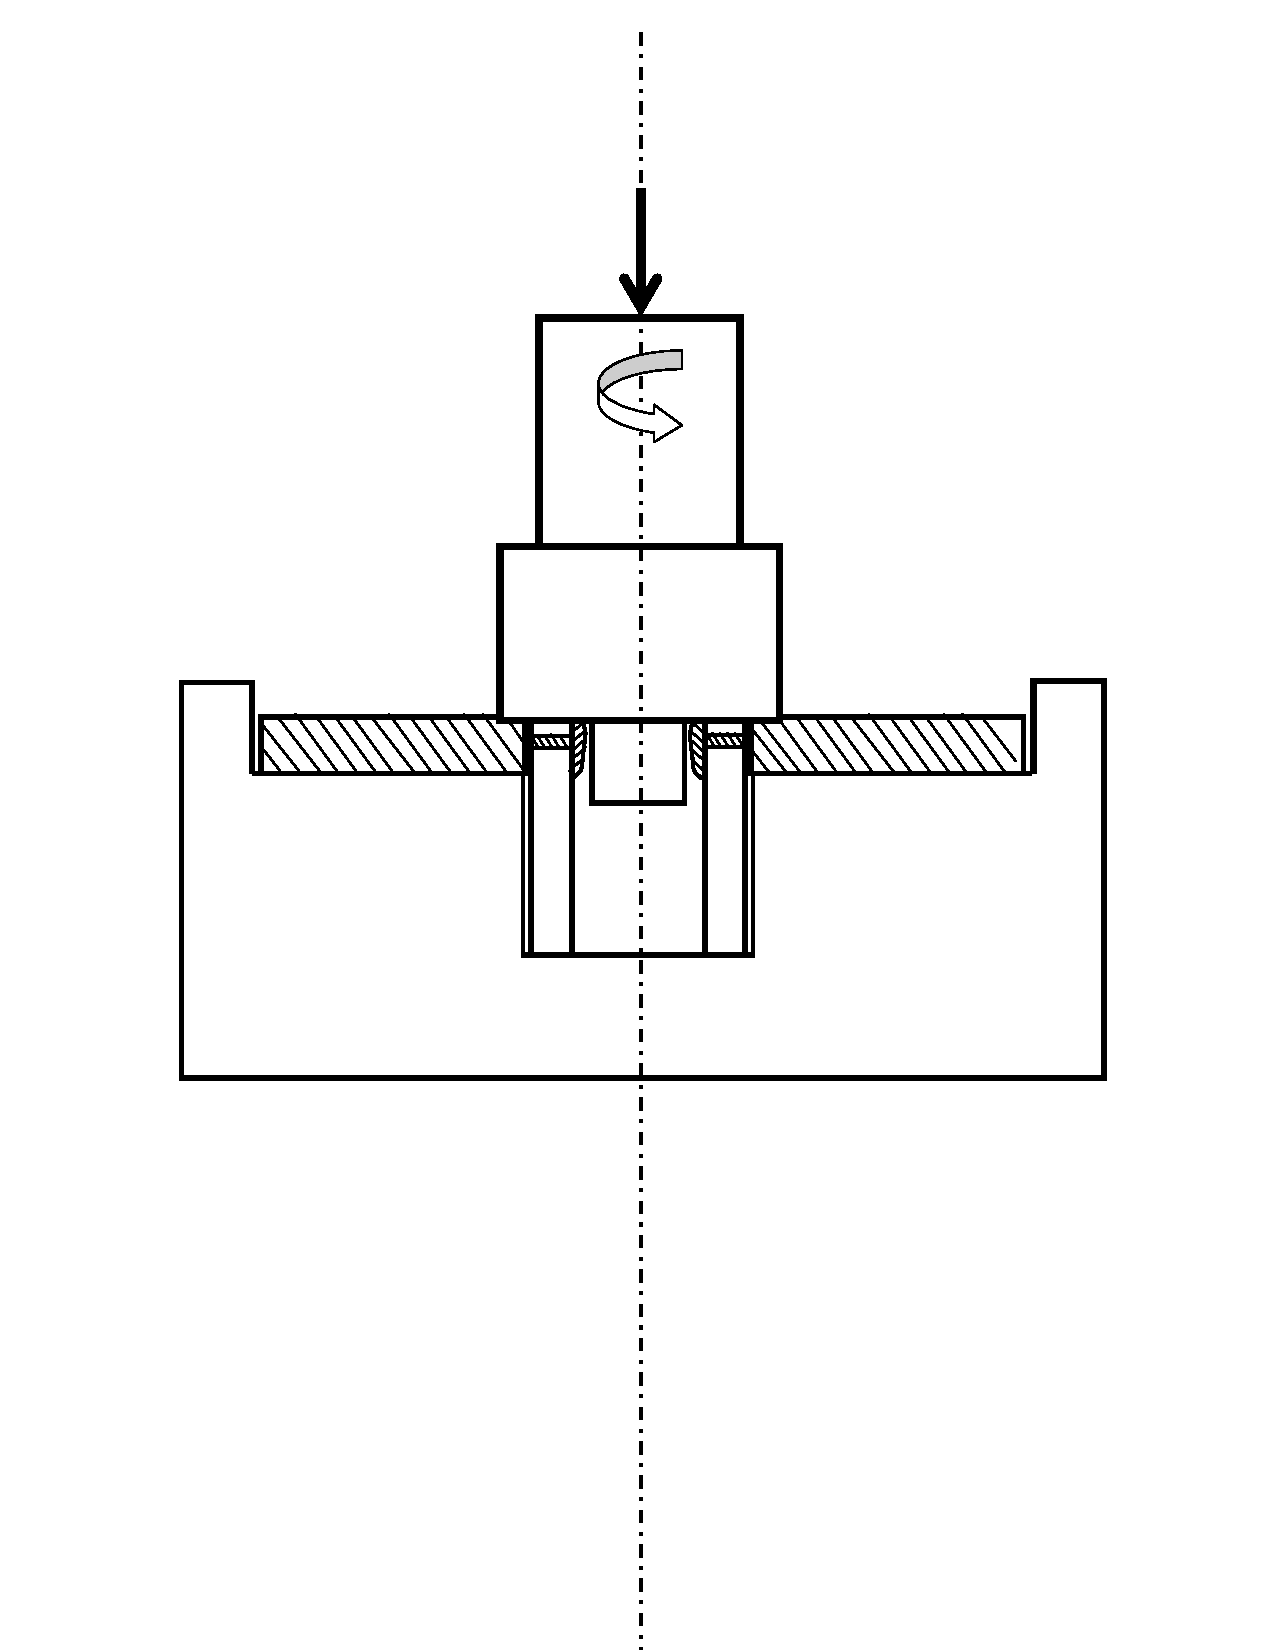
\includegraphics[trim=1cm 2cm 3cm 4cm, scale=0.1,width=\textwidth]{images/welding set up.pdf}
\caption{FWTPET Process}
\label{fig:fwtpet-process}
\end{figure}
\par 
Highest performance, concurrent weight and cost reduction has become more and more important in aviation industry. There are different approaches to meet these demands. It is well known, for example, that welding of skin-stringer joints is progressively replacing riveted fuselage structures. Another very effective possibility is the implementation of hybrid structures; components made of different materials can be tailored for local needs. There is a rising need for a welding method to join dissimilar materials, such as Titanium (Ti) and Aluminium (Al). However, joining of Al alloys to Ti alloys is difficult due to the formation of excessive intermetallic compounds at interface by traditional fusion welding method [1]. Excessive intermetallic compounds at the interface will make the joint brittle thereby reducing the weld strength. AA6061 is a low melting soft metal whereas Ti-6Al-4V is a high melting hard material. Welding a low melting alloy (AA6061) with a high temperature material (Ti-6Al-4V) is extremely difficult by conventional fusion welding process. This leads to lesser heat generation at interface and in turn leads to lesser intermetallic formation when compared to Friction Stir Welding (FSW) processes \cite{MadhusudhanReddy2009}.

%%%%%%%%%%%%%%%%%%%%%%%%%%%%%%%%%%%%%%%%%%Experimental Details%%%%%%%%%%%%%%%%%%%%%%%%%%%%%%%%%%%%%%

\section{Experimental Details} 
\label{sec:Experimental Details}
\subsection{Materials}
\label{subsec:Materials}
The materials used for welding were AA6061 tube plates and Titanium Grade V (Ti-6Al-4V) tubes. The base material composition of AA6061 is given in Table~\ref{table:AA6061-composition} and Ti-6Al-4V is given in Table~\ref{table:Ti-6Al-4V-composition}. The external tool used for welding was made of Tungsten alloy having 29mm shoulder diameter and 12.5 mm pin diameter. Chemical composition of the external tool is given in Table~\ref{table:tool-composition}. 
\par 
AA6061 plates of 6 mm thickness were cut into 50 x 50 mm squares. A hole of 19 mm diameter was drilled at the center of the plate. Ti-6Al-4V tube of with 19 mm outer diameter and 14 mm inner diameter were used for welding. Two tube profiles, holes and petals were used for welding.
\begin{enumerate}[1.]
\item Holes : Holes of 2 mm diameter were drilled at equal intervals along the circumference of the Ti-6Al-4V tubes of height 20 mm. The holes were made at a depth of 5 mm from top of the tube.
\item Petals : Slots of length 10 mm and width 2 mm were made at equal intervals along the circumference of the Ti-6Al-4V tubes of height 30 mm. The slots were then formed into petals using a suitable tool.
\end{enumerate}

\begin{table*}[!htbp]
\caption{CHEMICAL COMPOSITION OF Ti-6Al-4V}
\centering
\begin{tabular}{|c|c|c|c|c|c|c|c|c|c|}
\hline 
Element & C & Fe & O & N & Al & H & V & Y & Ti\\ 
\hline 
Wt \% & 0.08 & 0.03 & 0.2 & 0.05 & 0.148 & 5.5-6.75 & 3.5-4.5 & 0.005 & balance\\ 
\hline 
\end{tabular}
\label{table:Ti-6Al-4V-composition} % is used to refer this table in the text
\end{table*}


\begin{table*}[!htbp]
\caption{CHEMICAL COMPOSITION OF AA6061}
\centering
\begin{tabular}{|c|c|c|c|c|c|c|c|c|c|}
\hline 
Element & Mg & Si & Fe & Cu & Cr & Mn & Ti & Zn & Al\\ 
\hline 
Wt \% & 0.70 & 0.43 & 0.497 & 0.164 & 0.148 & 0.045 & 0.0495 & 0.0042 & balance\\ 
\hline 
\end{tabular}
\label{table:AA6061-composition} % is used to refer this table in the text
\end{table*}

\begin{table*}[!htbp]
\caption{CHEMICAL COMPOSITION OF TOOL MATERIAL}
\centering
\begin{tabular}{|c|c|c|c|c|c|}
\hline 
Element & W & Ni & Co & Fe & O \\ 
\hline 
Wt \% & 90.5 & 5.3 & 0.2 & 3.4 & 0.007 \\ 
\hline 
\end{tabular}
\label{table:tool-composition} % is used to refer this table in the text
\end{table*}

\subsection{FWTPET}
\label{subsec:FWTPET}
FWTPET process was carried out in a 4-Axis Friction Stir Welding machine (\ref{fig:fsw-machine}). Before welding, the tube and plate were cleaned with Acetone to remove dirt and grease. Then the tube and plate were fitted to a specially designed backing block as shown in \ref{fig:backing-block}. The parameter used for welding are given in Table \ref{table:process-parameters}. %The samples were welded at 4 different tool rotational speeds : 560, 710, 1120 and 1200 rpm. The parameters that were kept constant for all the welds were plunge rate - 2 mm/min, plunge depth - 2 mm and tube projection - 2 mm.

\begin{table*}[!htbp]
\caption{FWTPET Process Parameters}
\centering
\begin{tabular}{|c|c|}
\hline 
Plunge Depth & 2 mm \\ 
\hline 
Plunge Rate & 5 mm/min \\ 
\hline 
Tube Projection & 2 mm \\ 
\hline 
Tool Rotational Speed & 550, 700, 900, 1100 RPM \\ 
\hline 
\end{tabular} 
\label{table:process-parameters} % is used to refer this table in the text
\end{table*}

\subsection{Plunge Shear Test}
\label{subsec:Plunge Shear Test}
The joint strength of the welds were measured using an in-house developed testing procedure called ``Plunge Shear Test''. Plunge Shear Test (PST) is a destructive testing method which can be carried out on a conventional UTM with the help of an external plunger. In order to perform the PST, a specially designed half-solid and half-hollow tube must be used for welding as shown in Fig. After welding, the the sample is placed in a specially designed fixture and fixed to a UTM. With the help of a plunger (Fig.), a compressive load is applied on the solid part of the tube by the UTM, until the joint breaks.
\par
For our current work, for holes profile, a rod of 19 mm diameter and 30 mm length was taken and a hole of 14 mm diameter was drilled to a depth of 20 mm as shown in Fig. For petals profile, a rod of 19 mm diameter and 35 mm length was taken and a hole of 14 mm diameter was drilled to a depth of 20 mm as shown in Fig.


\subsection{Characterization}
\label{subsec:Characterization}
The welded samples were sectioned at the weld joint for metallographic studies. Studies were made using a standard stereoscope and optical microscope. SEM and EDS analysis were performed to quantify the elemental weight percentage at the joint interface. The observations were carried out in a 200kV field effect scanning electron microscope (SEM-JEOL JSM 5410LV microscopy) coupled with EDS. EDS line scan was also carried out along the weld interface. XRD analysis was done at the weld interface of Al-Ti dissimilar welds. XRD analysis helps to find out the formation of intermetallic at the weld interface. Scan speed was 10\degree /min and step width was 0.02\degree . In order to reveal the microstructures, a common etchant to etch both AA6061 and Ti-6Al-4V was developed. The etchant consists of equal parts of Ethanol, HCl, HNO$_{3}$ and few drops of HF. The etching time varied between 25 to 40 seconds based on the heat input on the welded samples.

%%%%%%%%%%%%%%%%%%%%%%%%%%%%%%%%%%%%%%%%%%Results and Discussion%%%%%%%%%%%%%%%%%%%%%%%%%%%%%%%%%%%%%%
\section{Results and Discussion}
\label{sec:Results and Discussion}

\subsection{Characterization}
\label{subsec:results-characterization}
The microstructure of AA6061-T651 base metal is shown in Fig. 6. Optical micrographs of the base AA6061-T6 revealed the presence of Mg$_{2}$Si precipitates which strengthens the Al
alloy [4]. After welding, AA6061-T6 showed fine grain structure at the weld interface with dissolution of Mg$_{2}$Si. In case of Ti-6Al-4V, the microstructure at the interface (Fig. 10) shows fine grain structure with equiaxed α phase with inter-granular retained β phase. When we move away from the interface, the
microstructure resembles that of the base metal microstructure for both AA6061-T651 and Ti-6Al-4V.After welding, AA6061-T651 showed fine grain structure at the weld interface with dissolution of Mg$_{2}$Si. In case of Ti-6Al-4V, the microstructure at the interface (Fig. 10) shows fine grain structure with equiaxed α phase with inter-granular retained β phase. When we move away from the interface, the microstructure resembles that of the base metal microstructure for both AA6061-T651 and Ti-6Al-4V.

\subsection{Weld Strength}
\label{subsec:Weld Strength}
In order to calculate the weld strength, the welded specimen should fail exactly at the joint interface. The fracture load of the weld joint when divided by the area of the weld gives the weld strength \ref{eq:weld-strength}. For FWTPET joints, the fracture load was measured using Plunge Shear Test (PST). PST was designed in such a way that the welded specimens fail exactly at the joint interface. For all speeds, the petals profile showed higher joint strength compared to the holes profile.  values for different tube profiles are given in Table II. From the table, it is clear that tube with petals is having high shear strength compared to other to profiles. This is due to the increase in weld area when compared to other tube profiles.
\begin{gather} \label{eq:weld-strength}
Weld\:Strength = \frac{\sigma}{A}
Weld\:Area &= \pi \: * d \: * \: h \\
\end{gather}

where~$\sigma$ is the fracture load and \\
~$A$ is the weld area. \\
~$d$ is the external diameter of the Ti-6Al-4V tube and \\
~$h$ is the height of weld.



\par

Fractography was done on both the Ti and Al side of the fractured samples. The river-flow pattern observed on the SEM images indicate that the joint failed by shear mode. All the welded samples failed at the joint.

\subsection{Heat Generated during FWTPET}
\label{subsec:Heat Generated during FWTPET}
\begin{gather} \label{eq:heat-input}
Q_{P} = \frac{2\pi}{3} *  w * \tau_{friction} * (R^{3}_{o} - R^{3}_{i})
\end{gather}
where~$Q_{P}$ is the Peak Heat generated at maximum load \\
$w$ is the ???? \\
$\tau_{friction}$ is the co-efficient of friction \\
$R_{o}$ is the outer radius and  \\
$R_{i}$ is the inner radius.

\subsection{X-Ray Diffraction Analysis}
\label{subsec:XRD-Results}
XRD plot at the weld interface for welds made with Tube with petals is shown in Fig. 12. From the XRD plot, the
presence of TiAl3 intermetallic formation was observed. Formation of intermetallic compounds is detrimental to joint strength. Titanium aluminide has three major intermetallic compounds: γ TiAl, α Ti$_{3}$Al and TiAl$_{3}$. Although these intermetallics have very good mechanical and thermal properties, they have very low ductility [6]. Therefore, the presence of Titanium aluminides at the interface might decrease the joint strength.

\begin{figure}[H]
\centering
\includegraphics[width=\textwidth]{images/xrd.png}
\caption{Tungsten Heavy Alloy Tool}
\label{fig:xrd-plot}
\end{figure}


\subsection{SEM Analysis}
\label{subsec:SEM Analysis}
SEM micrograph (Fig. 13) shows the Titanium particles entirely entrapped in the Al matrix at the weld interface. It can be seen that thick mixed layers are formed on the interface. EDS Line Scanning analysis was done along the interface. EDS patterns and element contents are shown in Fig. 14.

\subsection{Fractography}
\label{subsec:Fractography}
The SEM image (Fig. 15) shows fracture surface of Titanium tube for petal profile after the PST. From the image, we can clearly see some areas on the fracture surface where the aluminum alloy is still bonded to Titanium. SEM images of the fracture surface on the Aluminum plate shows cleavage facets, which is an indication shear fracture [7],[8]. Some Titanium particles embedded in the Aluminium matrix are also visible in
the SEM images (Fig. 16 b).

\section{Conclusion}
\label{sec:Conclusion}
\begin{enumerate}[1.]
\item FWTPET method has been established to join 6mm thick Aluminum (AA6061-T651) tube plate to Titanium (Ti-6Al-4V) tubes of 2.5mm wall thickness.
\item Three different tube profiles-hole, slot and petals, were used to study the feasibility of joining dissimilar materials (Al-Ti) using FWTPET and petal profile was found to have good strength.
\item Shear strength of the joint reached 60% of AA6061–T651 base material strength.
\item XRD analysis showed formation of TiAl3 at the interface. Intermetallic compounds at the interface were less when compared to traditional fusion welding processes which is due to the reduction in heat generation during the welding process.
\end{enumerate}

%%%%%%%%%%%%%%%%%%%%%%%%%%%%%%%%%%%%%%%%%%%%%%%%%%%%%%%%%%%%%%%%%%%%%%%%%%
							%%References
%% Following citation commands can be used in the body text:
%% Usage of \cite is as follows:
%%   \cite{key}         ==>>  [#]
%%   \cite[chap. 2]{key} ==>> [#, chap. 2]
%%

%%%%%%%%%%%%%%%%%%%%%%%%%%%%%%%%%%
%% Elsevier bibliography styles %%
%%%%%%%%%%%%%%%%%%%%%%%%%%%%%%%%%%
%% Numbered
%\bibliographystyle{model1-num-names}

%% Numbered without titles
%\bibliographystyle{model1a-num-names}

%% Harvard
%\bibliographystyle{model2-names.bst}\biboptions{authoryear}

%% Vancouver numbered
%\usepackage{numcompress}\bibliographystyle{model3-num-names}

%% Vancouver name/year
%\usepackage{numcompress}\bibliographystyle{model4-names}\biboptions{authoryear}

%% APA style
%\bibliographystyle{model5-names}\biboptions{authoryear}

%% AMA style
%\usepackage{numcompress}\bibliographystyle{model6-num-names}

%% `Elsevier LaTeX' style
\bibliographystyle{elsarticle-num}

%% References with BibTeX database:
%% Authors are advised to use a BibTeX database file for their reference list.
%% The provided style file elsarticle-num.bst formats references in the required style

\bibliography{bibtex-database}

%% For references without a BibTeX database:

% \begin{thebibliography}{00}

%% \bibitem must have the following form:
%%   \bibitem{key}...
%%

% \bibitem{}

% \end{thebibliography}
%%%%%%%%%%%%%%%%%%%%%%%%%%%%%%%%%%%%%%%%%%%%%%%%%%%%%%%%%%%%%%%%%%%%%%%%%%
							%%Appendix
%% The Appendices part is started with the command \appendix;
%% appendix sections are then done as normal sections
%% \appendix

\end{document}